\chapter{Navier-Stokes equation -- 2D -- Incompressible -- Driven Cavity}

\modinfo{Directory}{DrivenCavity}
\modinfo{Solvers}{\Idx{FlowSolve}}
\modinfo{Tools}{\Idx{ElmerGrid}, \Idx{ElmerGUI}}
\modinfo{Dimensions}{2D, Steady-state}
\modinfo{Author}{Evangelos Voyiatzis}


\subsection*{Introduction}

This simple tutorial illustrates the application of Elmer to computational fluid dynamics problems.
The computational mesh is generated using the ElmerGrid utility while the model definition and its solution are carried out via ElmerGUI. The results are visualized with ParaView.

\subsection*{Case definition}

The geometrical domain, which is shown in Figure \ref{fg:DC_geometry}, is a square with a side length of 1 m. The square is filled with an ideal fluid with a density of 1 kg/m\textsuperscript{3} and a viscosity of 0.01 kg/m s. The boundary $\Gamma_{A-B}$ is moving with a constant speed of 4 m/s in the x Cartesian direction while the no slip boundary condition is applied to the rest of the boundaries. The flow is laminar with a Reynolds number of 400. This system has been studied in detail by Ghia, Ghia and Shin in J. Comp. Phys. 48 (1982) 387-411 and it is also part of the NASA repository \url{https://www.grc.nasa.gov/WWW/wind/valid/cavity/cavity.html}.\\

The study by Ghia, et al, is run with a range of Reynolds numbers, from 100 up to 10,000.  We will examine the case of Reynolds number equal to 400.  Using SI units, the driven lid moves at 4 m/s, the viscosity equals 0.01 Pa-s, and the density equals 1.0 kg/m\^3.  The values are chosen to provide the desired Reynolds numbers from the Ghia article simply by changing the driven lid velocity.  For example, with the lid moving at 4 m/s we have a Reynolds number of 400, if the lid moves at 1 m/s we will have a Reynolds number of 100, and so forth.\\

The study by Ghia, et al, presents numerical results in two tables.  The tabular results are the u velocity (in the x-direction) along a vertical line through the geometrical center and the v velocity (in the y-direction) along a horizontal line through the geometrical center.  The two lines are shown in Figure \ref{fg:DC_geometry}.  A comparison of the tabulated results from Ghia against the results generated by Elmer will be presented.\\

\begin{figure}[H]
\centering
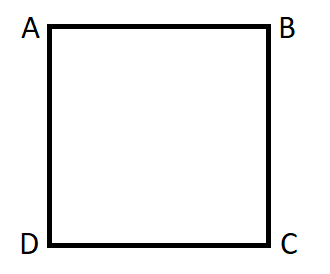
\includegraphics[scale=1.2]{DC_geometry}
\caption{Geometry of the driven cavity problem}\label{fg:DC_geometry}
\end{figure}  

Mathematically the problem to be solved is
\begin{equation}
\left \{
\begin{array}{rccl}
- \nabla \cdot (2 \mu \overline{\overline{\varepsilon}}) + \rho 
\vec{u} \cdot \nabla \vec{u} + \nabla p & = & 0 & \mbox{ in } \Omega \\
\nabla \cdot \vec{u} & = & 0 & \mbox{ in } \Omega \\
\end{array}
\right .
\end{equation}
%
with the boundary conditions
\begin{equation}
\left \{
\begin{array}{rccl}
u_x & = & 4 	 & \mbox{ on } \Gamma_{A-B} \\
u_x & = & 0 & \mbox{ on } \Gamma_{B-C} \cup \Gamma_{C-D} \cup \Gamma_{D-A} \\
u_y & = & 0 & \mbox{ on } \Gamma  
\end{array}
\right .
\end{equation}
where $\mu$ is the viscosity, $\overline{\overline{\varepsilon}}$ is 
the strain tensor,  $\rho$ is the density, $\vec{u}$ is the velocity and
$p$ is the pressure. It is assumed that the density and viscosity are 
constants. 

\subsection*{Solution procedure}

The first step is the generation of a uniform computational mesh with 128 elements in each of the x and the y coordinate directions. This is achieved by the following input file for ElmerGrid which is stored in the "DrivenCavity.grd" file, which may be found in the tutorials-GUI-files/DrivenCavity folder:

\ttbegin
*** ElmerGrid input file for structured grid generation ***
Version = 210903
Coordinate System = Cartesian 2D
Subcell Divisions in 2D = 1 1
Subcell Limits 1 = 0 1
Subcell Limits 2 = 0 1
Material Structure in 2D
  1
End
Materials Interval = 1 1
Boundary Definitions
! type out int double of the boundaries
  1     -1   1   1
  2     -2   1   1
  3     -3   1   1
  4     -4   1   1
End
Element Degree = 2
Surface Elements = 16384
\ttend

Then start ElmerGUI and create a new project, as follows:

\begin{verbatim}
Run
  New Project...
\end{verbatim}

Start at the top and select the project directory as shown in Figure \ref{fg:new_project}.  Then select the Geometry input file, DrivenCavity.grd.  Lastly, the SaveLine Equation Definition File is needed for the tutorial, so select SaveLine in the right hand box and add it to the left hand box.  Click on OK to accept the changes.

\begin{figure}[H]
\centering
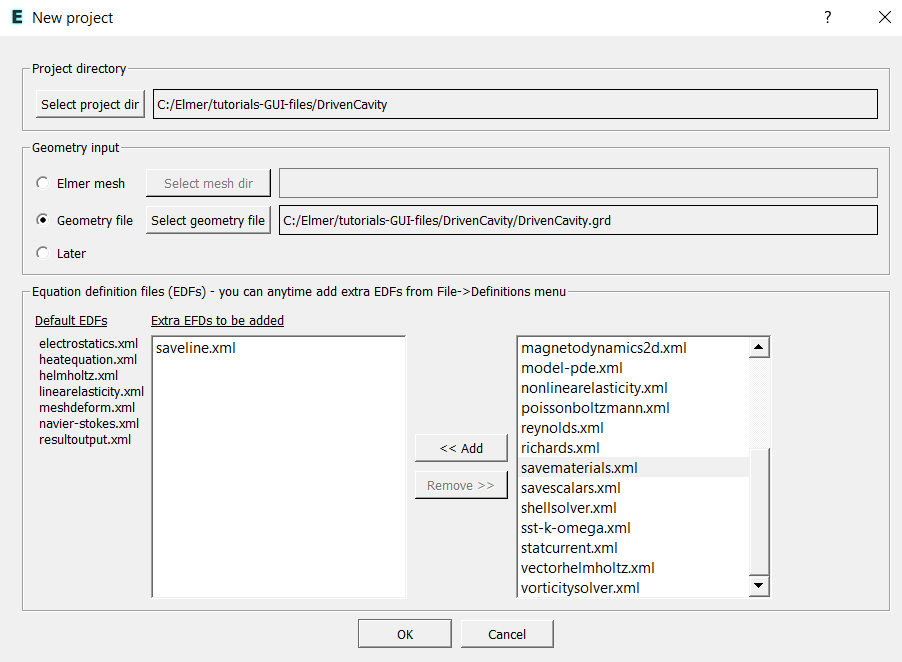
\includegraphics[width=0.9\textwidth]{new_project.png}
\caption{New Project}\label{fg:new_project}
\end{figure}  

\subsection*{ElmerGUI Equation Definition Files}

The New Project screen automatically locates and lists all of the available EDFs.  The left side of the screen lists the Default EDFs, which will be loaded into each ElmerGUI project.  The right hand box lists all of the extra EDFs, that are not normally loaded, allowing the option to add individual extra EDFs to a new project.\\

This tutorial will use the Default EDF, \texttt{\Idx{navier-stokes.xml}}, for the \Idx{Navier-Stokes Solver}.  In addition, we will add the Extra EDF,  \texttt{\Idx{saveline.xml}}, for the \Idx{SaveLine Solver}.

Finish by clicking on OK.  ElmerGUI will generate a mesh which is visualized in Figure \ref{fg:DC_mesh}.

\begin{figure}[H]
\centering
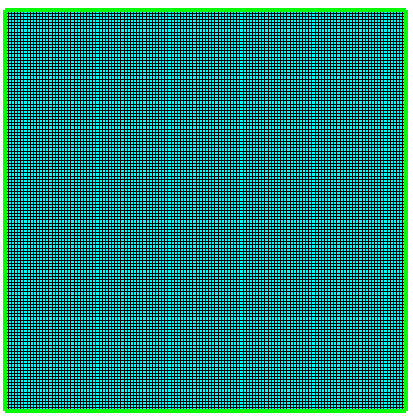
\includegraphics[scale=0.6]{DC_mesh}
\caption{The mesh for the driven cavity problem}\label{fg:DC_mesh}
\end{figure}

You can verify that the mesh consists of 16384 surface elements by inspecting the dialog box that appears when selecting

\ttbegin
Model
  Summary
\ttend

We can now define the model going through the Model menu from the top to bottom.  
In the equation section we choose the relevant equations and parameters related to their solution. 
We have only one set of equations which consists of the incompressible Navier-Stokes equation.
We also will use the SaveLine tab in the equations menu.

\ttbegin
Model
  Equation -> Add ..
\ttend  

We select the Navier-Stokes tab, click on the `Active' box, and click to apply the equation to `Body 1'.
We will accept the default settings for the Navier-Stokes equation for now.

Since we have two solvers active for Body 1, you may ask, which solver will run first and which solver
will run second?  Elmer has the ability to control when each solver will run.  For example, we could add
a priority number to each solver, where the higher priority number solver will run first.  In this case,
we want the Saveline solver to run after the Navier-Stokes solver has run.  While on the Navier-Stokes
tab, enter `2' in the priority box, then switch to the Saveline tab and enter `1' in the priority box.  Now the Navier-Stokes solver has the higher (numerically larger) priority number, so it will execute before the Saveline solver.\\

While on the SaveLine tab, click on the `Active' box.  Verify that `Body 1' is already selected.  Don't click
on the `OK' button just yet, we still need to add some info into the Saveline solver.\\

The equation tabs should look like Figure \ref{fg:DC_equation}. 

\begin{figure}[H]
\centering
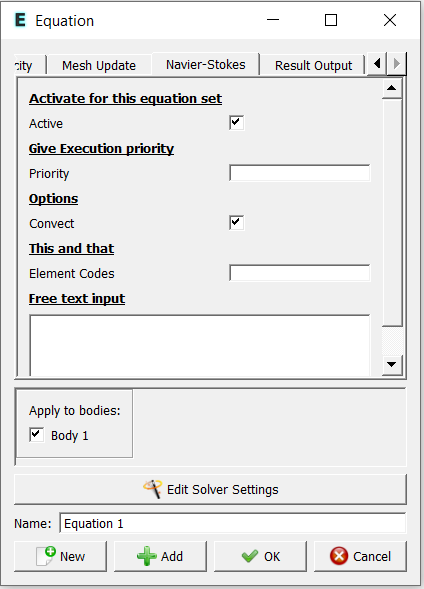
\includegraphics[width=0.48\textwidth]{DC_equation}
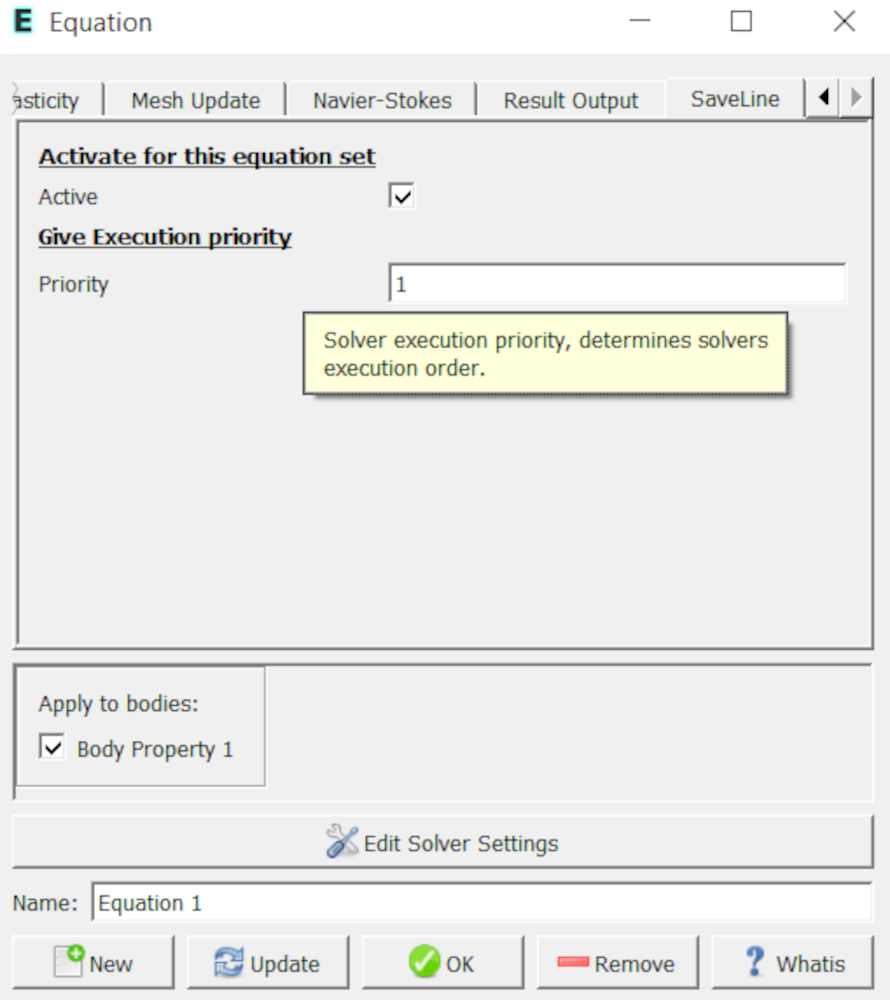
\includegraphics[width=0.48\textwidth]{DC_equation2}
\caption{Activate Equations, Navier-Stokes on left, Saveline on right}\label{fg:DC_equation}
\end{figure}

While the SaveLine tab is active, click on the `Edit Solver Settings' tab, followed by the
`Solver specific options' tab, and enter the information below as shown.  Saveline needs to
know what name to use when it creates the results file, in this case, we will enter
`save-400.dat'.  For \Idx{Polyline Coordinates} and for \Idx{Polyline Divisions}, enter

\ttbegin
Size(4,2); 0.5 1.0 0.5 0.0 1.0 0.5 0.0 0.5
Size(2);20 20
\ttend  

The SaveLine tab should look like Figure \ref{fg:DC_saveline}.  Now finish up by clicking
on the `OK' button to close the Equation menu.

In a later section we will discuss the details of creating the SaveLine settings.

\begin{figure}[H]
\centering
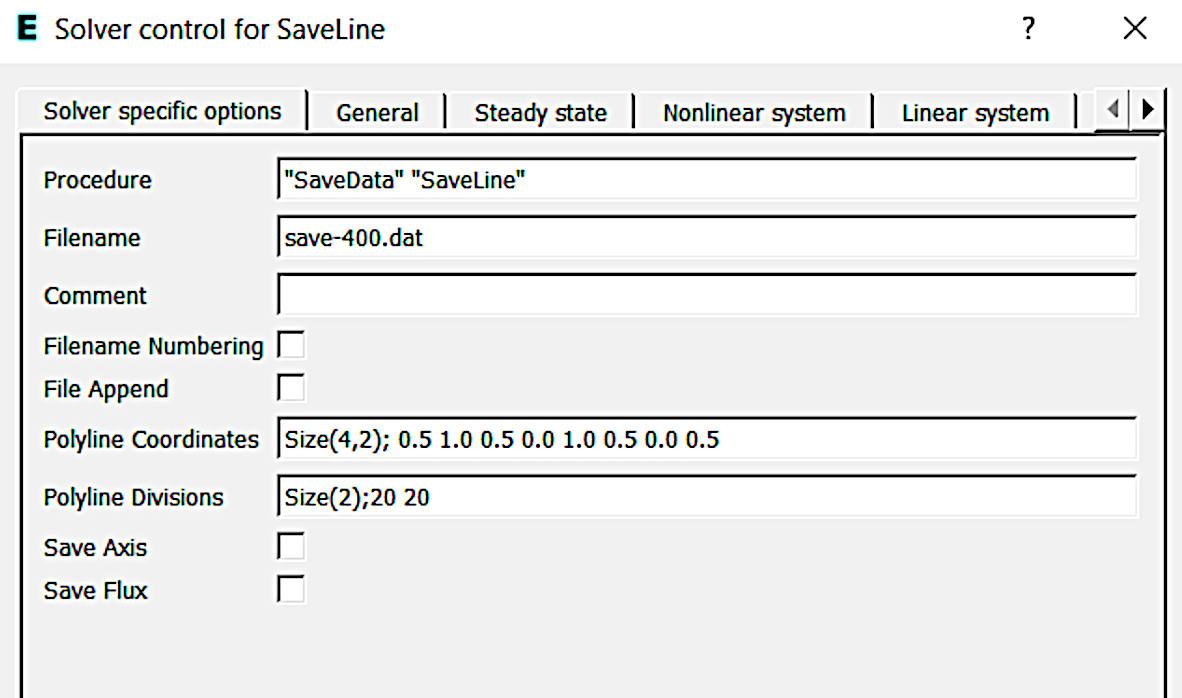
\includegraphics[scale=1.3]{DC_saveline}
\caption{SaveLine Specific Settings}\label{fg:DC_saveline}
\end{figure}

\newpage
The Material section includes all material parameters. They are divided into generic parameters which are direct properties of the material without making any assumptions on the physical model, such as the density. Other properties assume a physical law, such as the viscosity. 
In the material section, we select 

\ttbegin
Model
  Material -> Add .. 
\ttend  

The Material menu allows entry of any desired material properties, or one could select pre-defined
materials from the `Material Library' button.  In our case, we will enter the material values as stated
under `Case Definition' above.

In the dialog box that appears, we first click on the General tab and we set the density equal to 1 and apply it to "Body 1" as shown in left panel of Figure \ref{fg:DC_material}.
Subsequently, we select the "Navier-Stokes" tab where we set the viscosity to 0.01, the "Compressibility model" to "Incompressible", apply it to "Body 1" and click ok as shown in the right panel of Figure \ref{fg:DC_material}.

\begin{figure}[H]
\centering
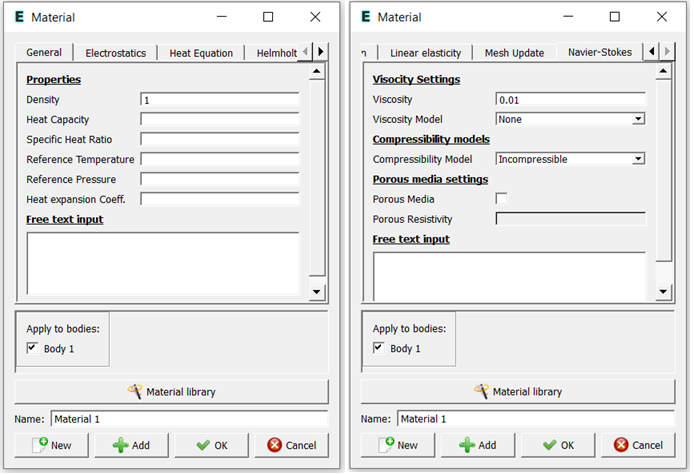
\includegraphics[width=0.8\textwidth]{DC_material}
\caption{Material properties}\label{fg:DC_material}
\end{figure}

For the linear system solvers we are happy to use the defaults. One may however, try out different preconditioners (ILU1,\ldots) or direct Umfpack solver, for example.

The appropriate boundary conditions can be set via  

\ttbegin
Model
  Boundary condition -> Add ..
\ttend

In the dialog box that appears, we select the "Navier-Stokes" tab. 
For boundary condition 1, we apply the no slip condition on boundaries 1, 2 and 4 by clicking on the
"No wall slip BC" option in the Navier-Stokes tab as shown in the left panel of Figure \ref{fg:DC_boundary}. 
For boundary condition 2, we apply the lid velocity with 4 m/s in the x-direction and 0 m/s in the y-direction  in the same tab after selecting "Boundary 3" as shown in the right panel of Figure \ref{fg:DC_boundary}.

\begin{figure}[H]
\centering
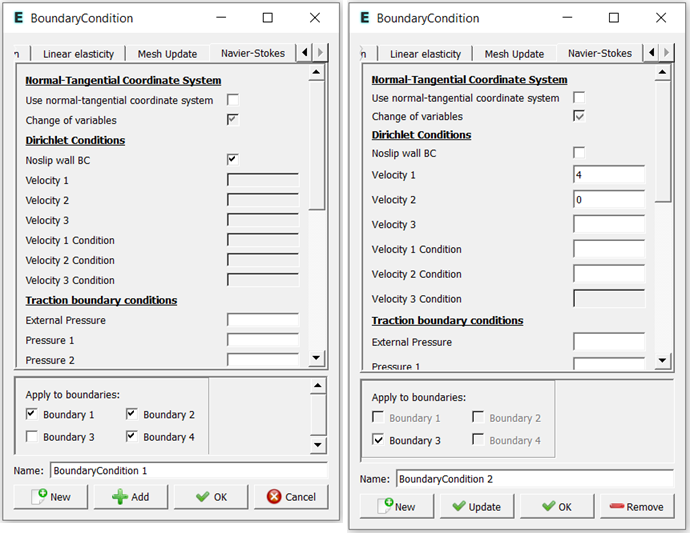
\includegraphics[width=0.8\textwidth]{DC_boundary}
\caption{Boundary conditions for the driven cavity}\label{fg:DC_boundary}
\end{figure}


For the execution, ElmerSolver needs the mesh files and the command file.  We can write and view the command file by selecting

\ttbegin
Sif 
  Generate
  Edit -> look how your command file came out  
\ttend

Before we can execute the solver we should save the files in a directory.  The ElmerGUI project includes all the files needed to restart the case.

\ttbegin
File 
  Save Project
\ttend

After we have successfully saved the files we may start the solver.

\ttbegin
Run
  Start solver
\ttend

A convergence view automatically pops up showing relative changes of each iteration. The problem should converge in less than ten iterations.
The variation of the residuals should be similar to the one in Figure \ref{fg:DC_convergence}. The required computational time should be a couple of minutes.

\begin{figure}[H]
\centering
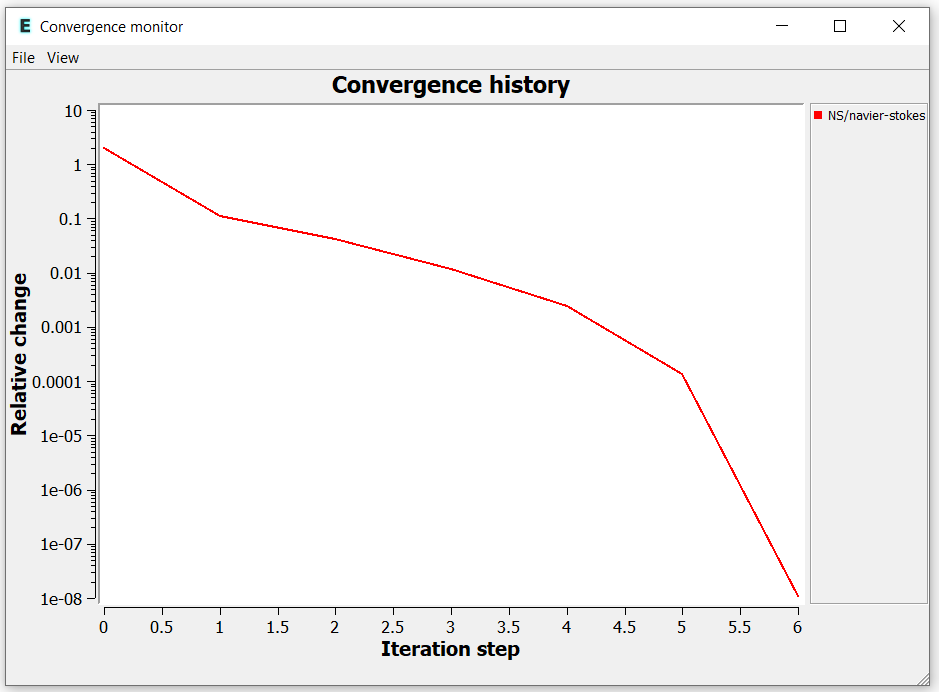
\includegraphics[scale=0.5]{DC_convergence}
\caption{Convergence of the solver.}\label{fg:DC_convergence}
\end{figure} 

When there are some results to view we may start the postprocessor:

\ttbegin
Run
  Start ParaView
\ttend
or
\ttbegin
Run
  Start ElmerVTK
\ttend

\subsection*{Graphical Results}

You may visualize the results with Paraview and/or ElmerVTK.  Results from each of the postprocessors
is shown, with the Paraview results on the left and the ElmerVTK results on the right.
In Figure \ref{fg:DC_velocity_magnitude} the magnitude of the obtained velocity field is presented.
The x- and y- cartesian components of the velocity vectors are shown in Figure \ref{fg:DC_velocity_x} and \ref{fg:DC_velocity_y}, respectively.\\

The results for the case of Reynolds number = 400 are shown in Figure \ref{fg:DC_velocity_magnitude},
Figure \ref{fg:DC_velocity_x}, and Figure \ref{fg:DC_velocity_y}.


\begin{figure}[H]
\centering
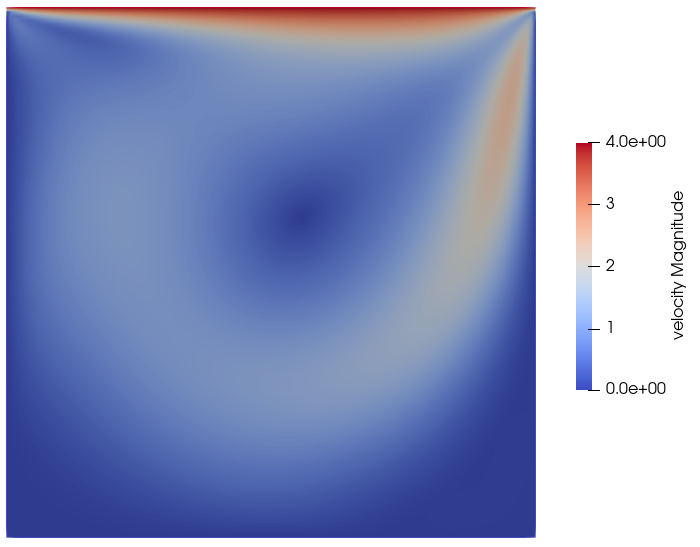
\includegraphics[scale=0.27]{DC_velocity_magnitude}
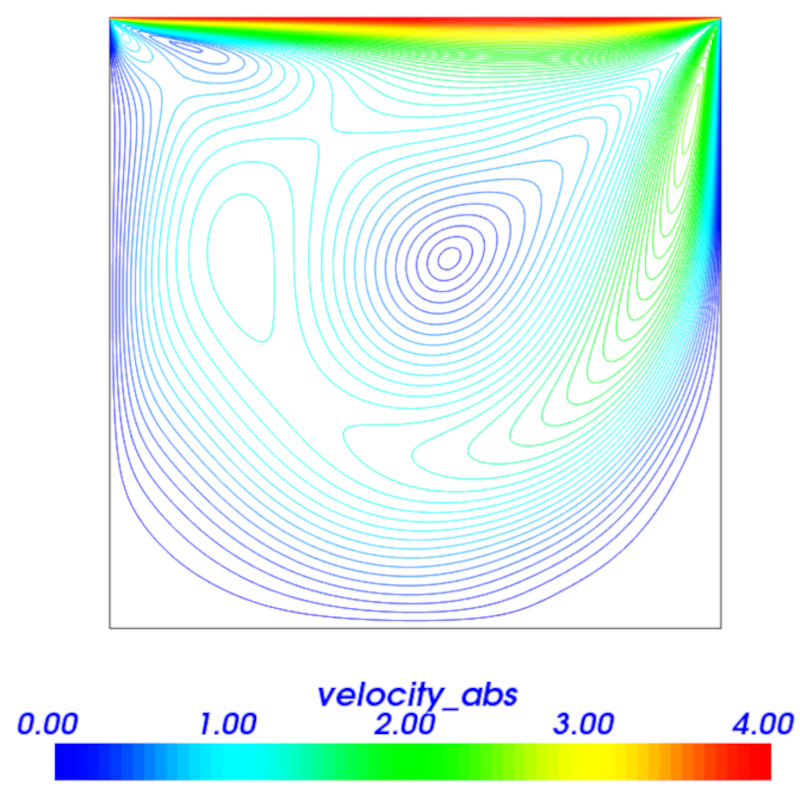
\includegraphics[scale=0.35]{DC_velocity_mag_VTK}
\caption{Re 400: Distribution of the magnitude of the velocity vector.}\label{fg:DC_velocity_magnitude}
\end{figure} 

\begin{figure}[H]
\centering
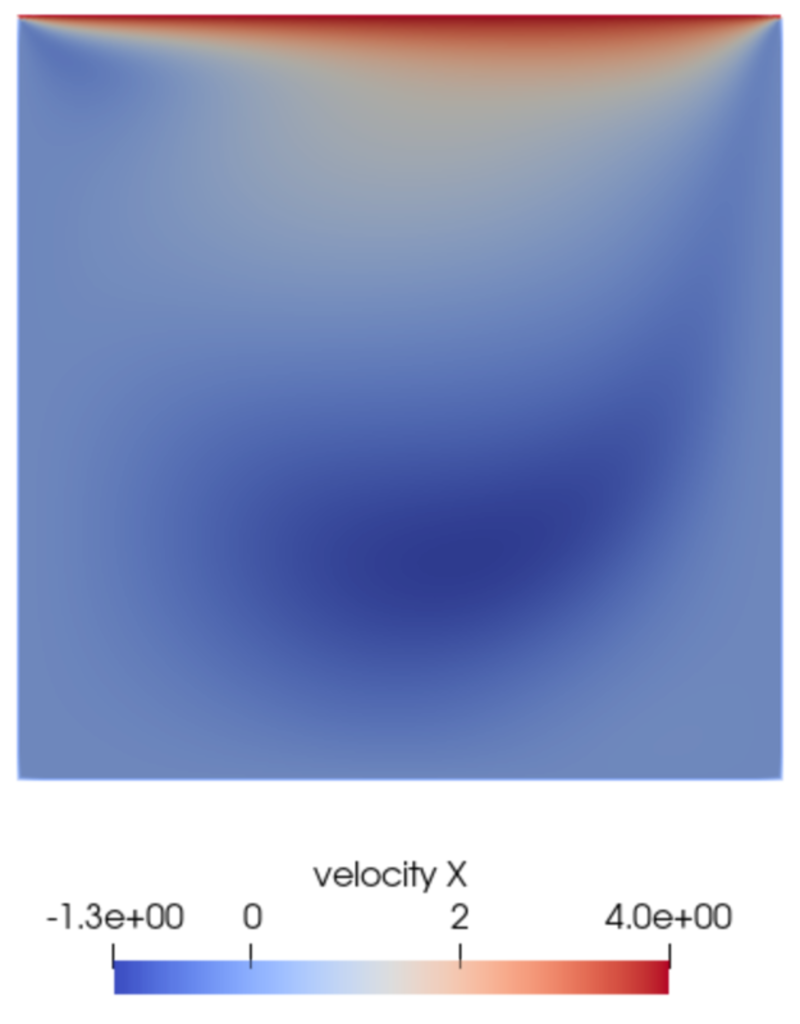
\includegraphics[scale=0.28]{DC_velocity_x}
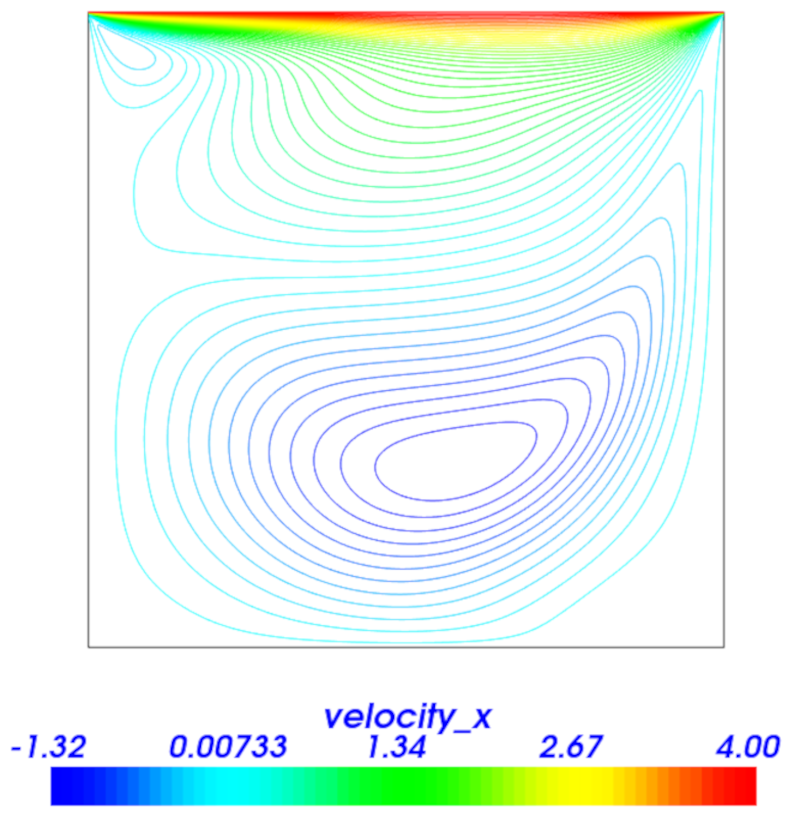
\includegraphics[scale=0.35]{DC_velocity_x_VTK}
\caption{Re 400: Distribution of x component of the velocity vector.}\label{fg:DC_velocity_x}
\end{figure} 

\begin{figure}[H]
\centering
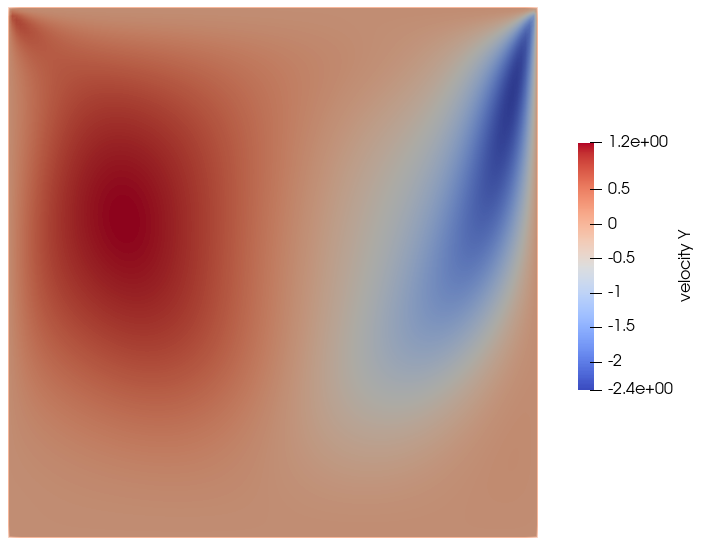
\includegraphics[scale=0.28]{DC_velocity_y}
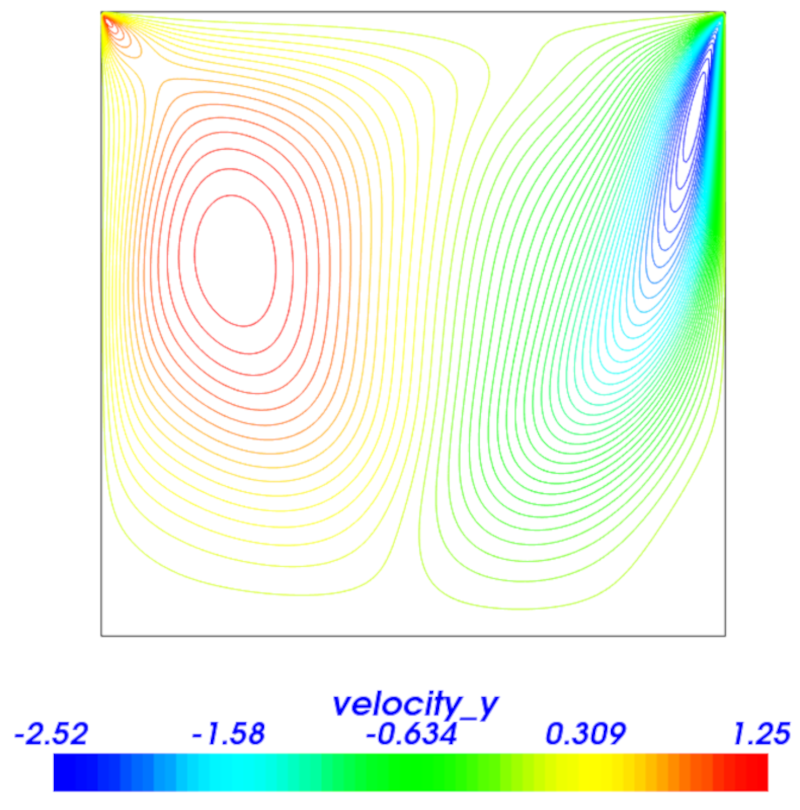
\includegraphics[scale=0.35]{DC_velocity_y_VTK}
\caption{Re 400: Distribution of y component of the velocity vector.}\label{fg:DC_velocity_y}
\end{figure} 

\subsection*{SaveLine}

The SaveLine subroutine contained in the SaveData solver is used to save Elmer solution data in ASCII format
along a line segment running through a 2D or 3D geometry model.  The SaveLine subroutine and keywords are described in
detail in the Elmer Models Manual.

The ElmerGUI equation tab for SaveLine was previously shown in Figure \ref{fg:DC_saveline}.  We entered data in
several of the fields, such as Filename, Polyline Coordinates, and Polyline Divisions.

For Filename, enter a descriptive name such as `save-400.dat', which indicates the Reynolds number 400 case,
with an extension such as `dat' or `csv'.  The file name and extension can be freely chosen.

Filename Numbering and File Append are not used for this case, but can be used when multiple simulation runs
are performed, such as a transient simulation.

Polyline Coordinates and Polyline Divisions are described in the Elmer Models Manual as follows:

\ttbegin
Polyline Coordinates(n,DIM) Real
  Save the line consisting of line segments defined by two points (n = 2).
  There can be more than one set of points (n = 2; 4; 6; : : :) but as a
  line segment is defined by two points there must be an even number of points.
Polyline Divisions(n/2,DIM) Integer
  The user may give the number of divisions for each polyline. This allows
  also the proper saving of discontinuous data. The size of this vector should
  be such that it is compatible with the number of lines.
\ttend

Polylines could also be called `Multiple Line Segments', because two end points must be defined for
each line segment.  For one line segment, two points, for two line segments, four points, etc.
Each point has the number of coordinates defined by the simulation, two coordinates for 2D and
three coordinates for 3D.  

In this case, we are dealing with a 2D simulation, so there will be two coordinates with DIM = 2.
The Ghia, et al, article presents tabular data for a vertical line and a horizontal line, both of which
pass through the geometric center.  We will need to define two line segments with four points,
so `n' = 4.  If we multiply n * DIM, (4*2=8) then we get the number of individual real numbers
that must be listed.  

Refer back to Figure \ref{fg:DC_saveline} and in the Polyline Coordinate entry box you will
see `Size(4,2);' which defines `n' and `DIM', followed by a series of eight numbers.

The Polyline Divisions entry box contains `Size(2);', where we enter `n/2', (4/2=2), followed by
two numbers, one for each line segment.  Each number indicates how many division are desired
for each line segment.  So if we want data results printed for a desired number of points along each
line segment, enter that number here.  In this case, we want twenty points along each line
segment.  On the other hand, if there is a sharp curve in the line segment that we want to
capture, dividing the line segment into 50 or 100 pieces, or splitting the single line segment into
three line segments with different divisions, will help add detail when we want to graph the results.

\subsection*{SaveLine Results}

\begin{figure}[H]
\centering
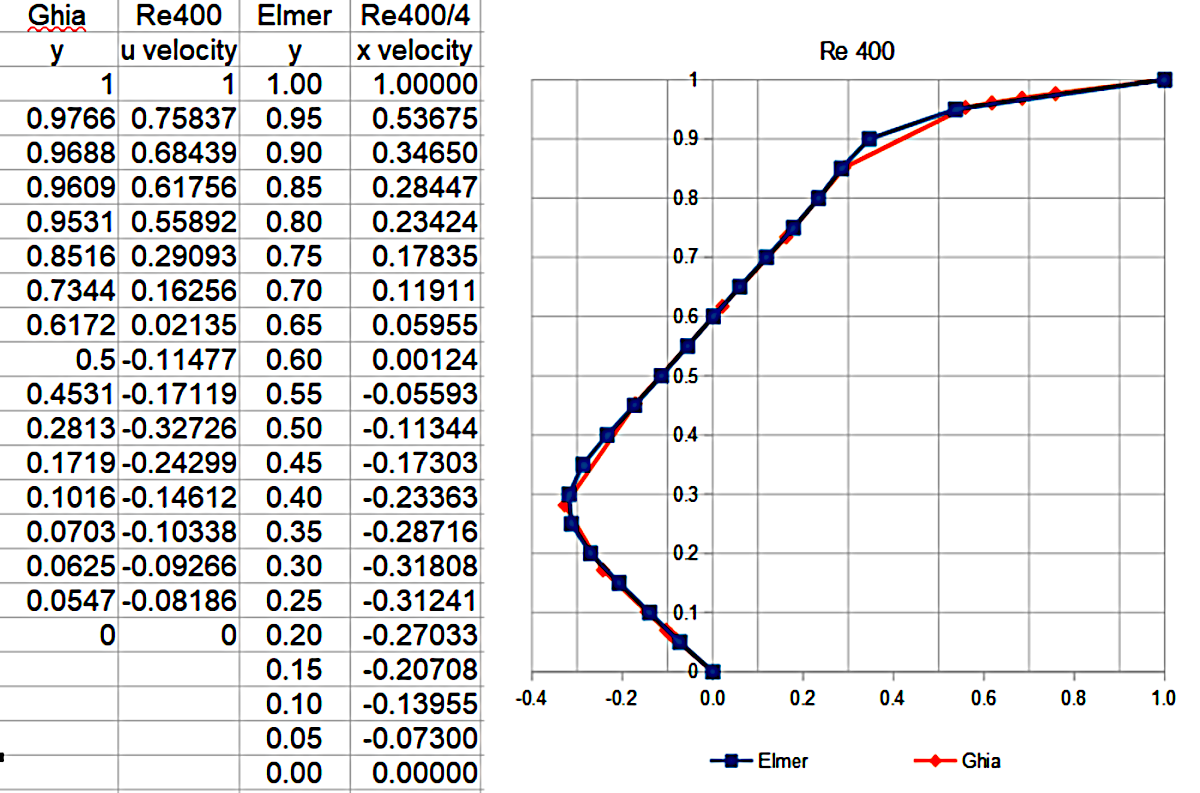
\includegraphics[scale=1.3]{Re400_compare}
\caption{Results comparison for Re = 400}\label{fg:results-400}
\end{figure} 

The left side of the spreadsheet presents the u velocity data from Table 1 in Ghia, et al, and
the right side of the spreadsheet presents the results calculated by Elmer.

The Elmer results must be normalized to between 0.0 and 1.0, by dividing by the
driven wall velocity, in this case divided by 4.

There is decent agreement between the two sets of results with a Reynolds number of 400.\\

\subsection*{High Reynolds Numbers}

The article by Ghia, et al, presents data over a range of Reynolds number.  The actual values
in the article are 100, 400, 1000, 3200, 5000, 7500, and 10,000.  You may try to solve the cases
with parameters corresponding to the given list of Reynolds numbers.  This can be achieved by
modifying the velocity of the upper boundary from 1 m/s up to 100 m/s, respectively.

Furthermore, although not shown in this tutorial, you can compare the obtained results
with the data from the NASA repository at \url{https://www.grc.nasa.gov/www/wind/valid/cavity/cavity.html}.

When running the range of Reynolds numbers, one will notice that starting at 50 m/s driven
velocity the solution will no longer converge when using the default solver settings.  Convergence
can be achieved up to the maximum speed of 100 m/s, Reynolds number of 10,000, by changing the
Navier-Stokes solver settings.

The Elmer Models Manual describes the details behind each of the documented solvers.
The Navier-Stokes Flow Solver is used for this driven cavity tutorial.  Increasing the Reynolds
number to 10,000 leads to issues with convergence.  The Linearization section of the Flow
Solver chapter mentions: `... to first take a couple of Picard iterations, and
switch to Newton iteration after the convergence has begun.'  In this case, increasing the
number of Picard iterations from 3 to 20, allows for convergence of the solution.
One other setting change is needed for convergence in this situation, and
that is to change from iterative to direct (umfpack) on the Linear tab.


\ttbegin
Model
  Equation
    Equation 1
      select the Navier-Stokes tab
      Edit Solver Settings
      select the Linear system tab
        click on the direct button under Method
        select Umfpack as the direct solver
      select the Nonlinear system tab
      Newton After iterations
        change from 3 to 20
      Apply
    Update
  OK
\ttend

For the case of Reynolds number = 10,000, velocity profiles are shown in Figures \ref{fg:DC_velocity_magnitude_10k}, \ref{fg:DC_velocity_x_10k} and  \ref{fg:DC_velocity_y_10k}.

\begin{figure}[H]
\centering
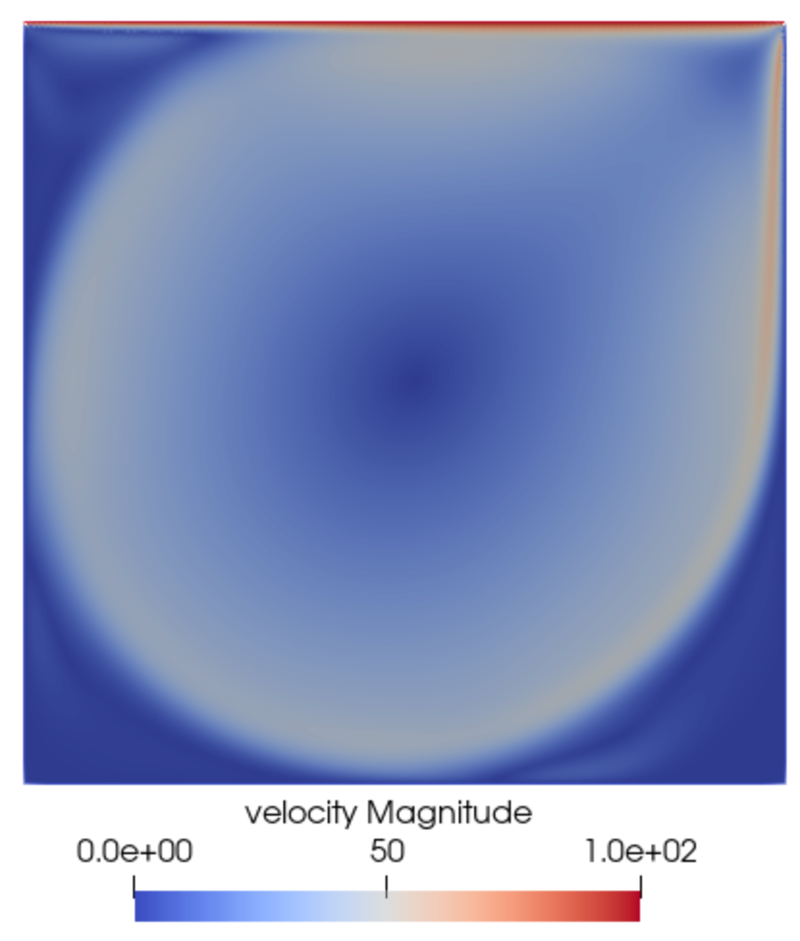
\includegraphics[width=0.43\textwidth]{DC_velocity_magnitude_10k}
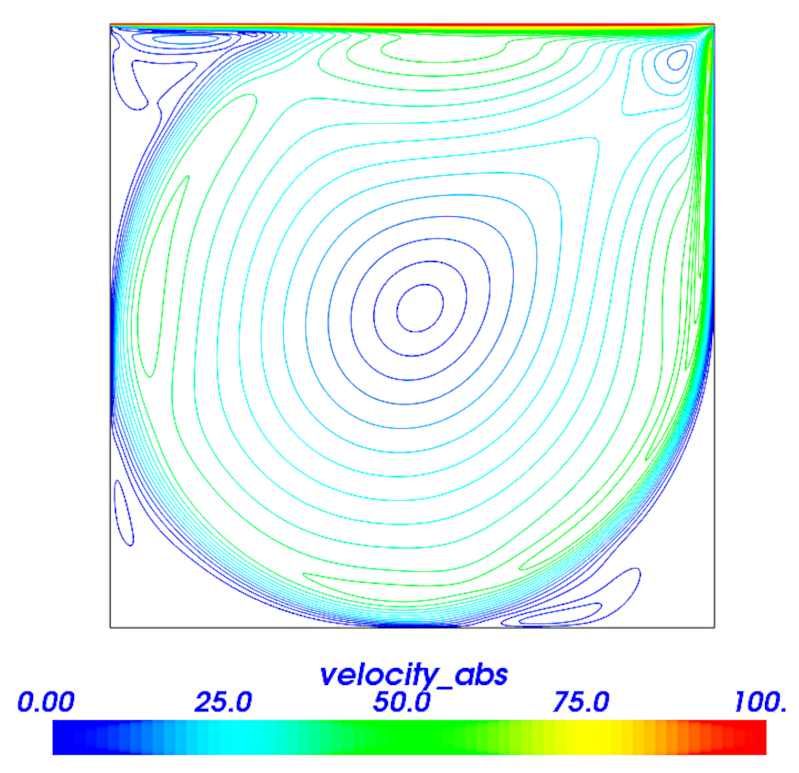
\includegraphics[width=0.54\textwidth]{DC_velocity_mag_VTK_10k}
\caption{Re 10,000: Distribution of the magnitude of the velocity vector.}\label{fg:DC_velocity_magnitude_10k}
\end{figure} 

\begin{figure}[H]
\centering
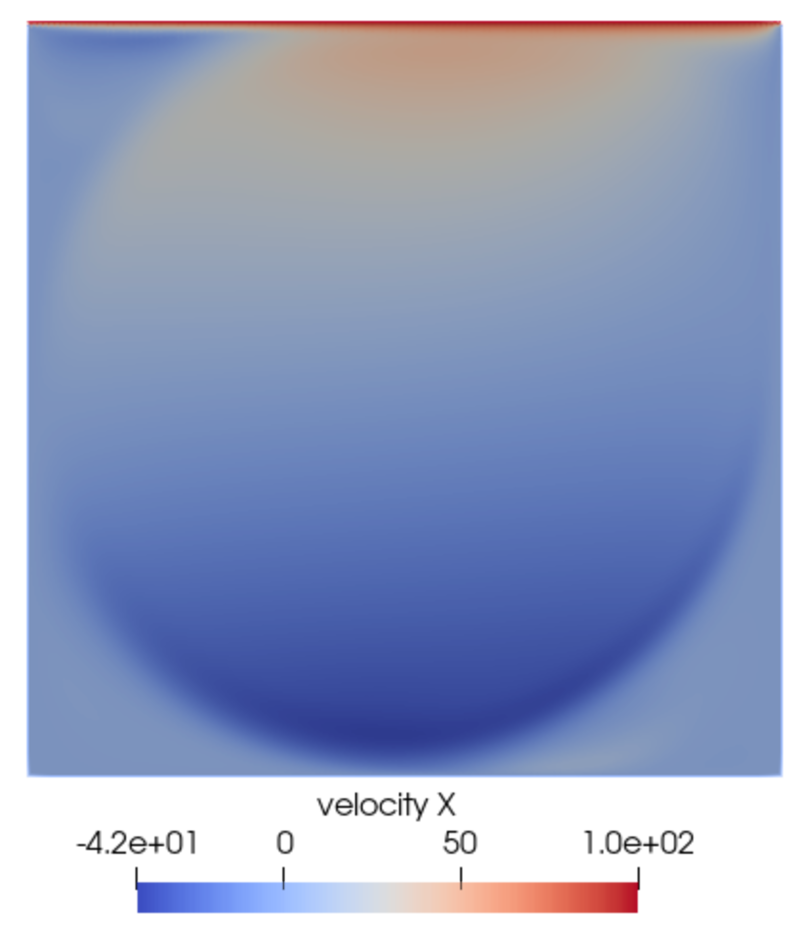
\includegraphics[width=0.43\textwidth]{DC_velocity_x_10k}
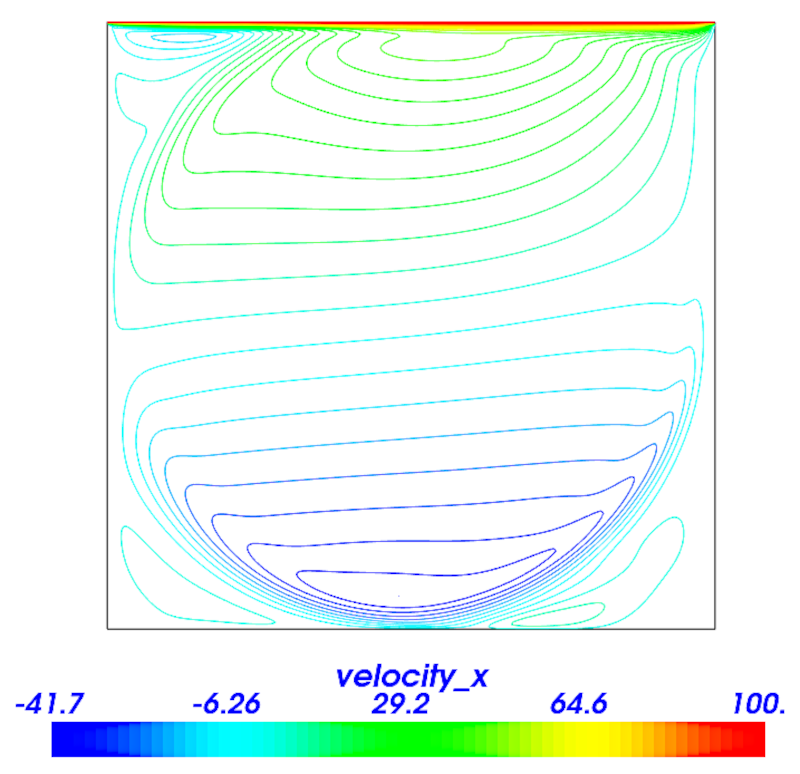
\includegraphics[width=0.54\textwidth]{DC_velocity_x_VTK_10k}
\caption{Re 10,000: Distribution of x component of the velocity vector.}\label{fg:DC_velocity_x_10k}
\end{figure} 

\begin{figure}[H]
\centering
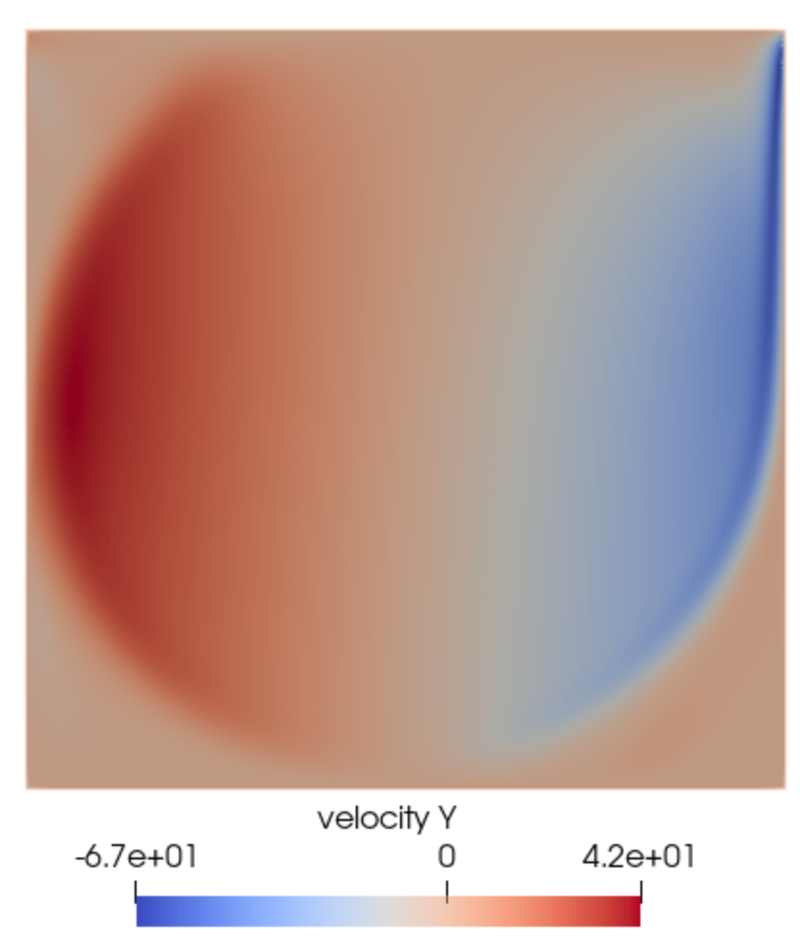
\includegraphics[width=0.43\textwidth]{DC_velocity_y_10k}
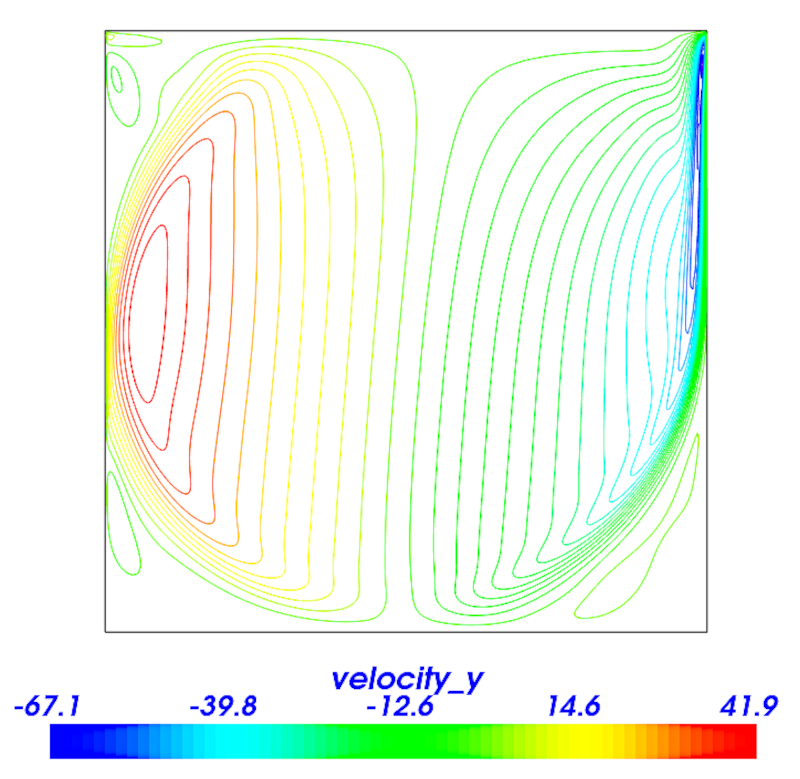
\includegraphics[width=0.54\textwidth]{DC_velocity_y_VTK_10k}
\caption{Re 10,000: Distribution of y component of the velocity vector.}\label{fg:DC_velocity_y_10k}
\end{figure} 

\newpage
Saveline results for the case with Reynolds number = 10,000 are shown in Figures \ref{fg:Re10k_u}
and  \ref{fg:Re10k_v}.  Some deviation between Elmer results and Ghia results can be observed
at the high Reynolds number case.  Overall, the shape of the curves of the results
show good agreement.

\begin{figure}[H]
\centering
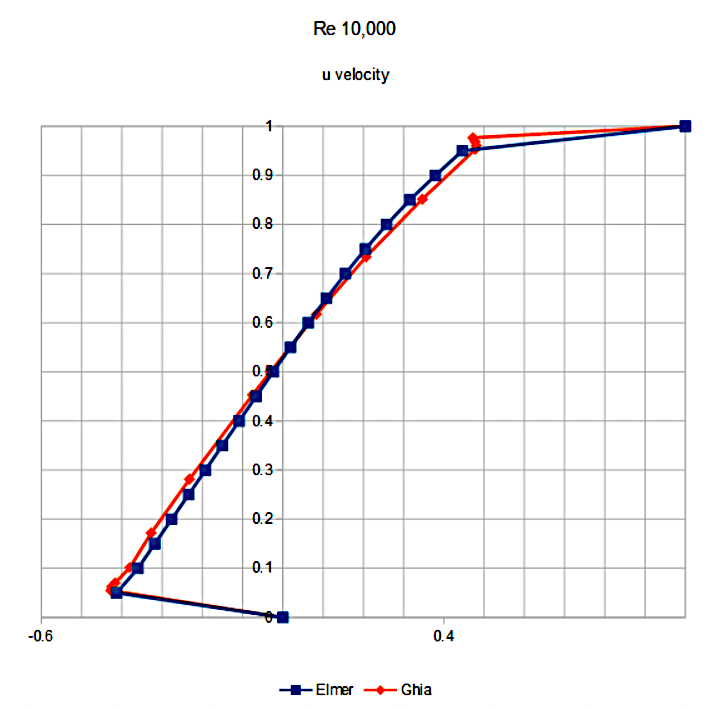
\includegraphics[scale=1.4]{Re10k_u}
\caption{Re 10,000 u velocity profiles}\label{fg:Re10k_u}
\end{figure} 

\begin{figure}[H]
\centering
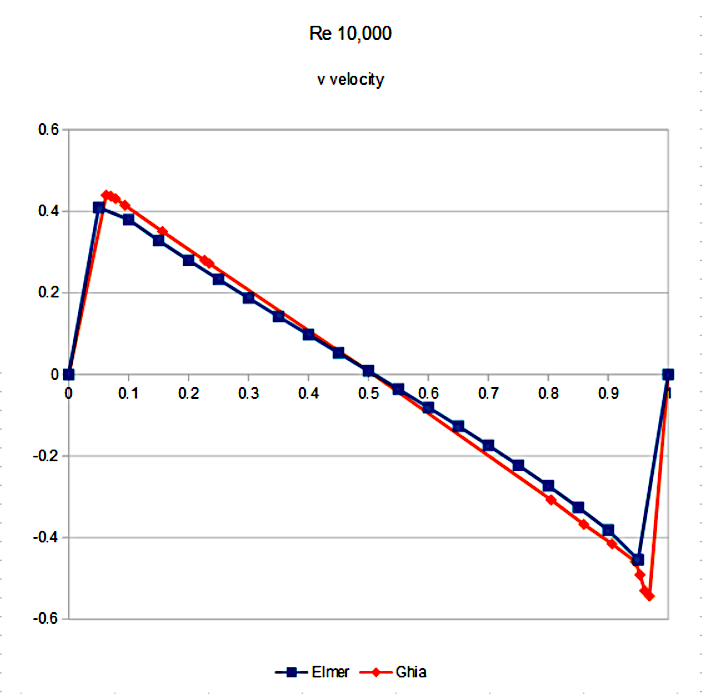
\includegraphics[scale=1.4]{Re10k_v}
\caption{Re 10,000 v velocity profiles}\label{fg:Re10k_v}
\end{figure} 

\subsection*{Extra task:}

For additional credit, try increasing the Reynolds number above 10,000.  For example, the solution will converge at Re = 20,000, if the non-linear relaxation factor is reduced from 1.0 to 0.7.
\hfill